% Passover Seder Liturgy
\documentclass[10pt,oneside,footinclude=true,headinclude=true]{scrbook} % KOMA-Script book
\usepackage[LHE,T1]{fontenc}
%\usepackage{lipsum}
\usepackage[linedheaders,manychapters,parts]{classicthesis} % ,manychapters
%\usepackage[osf]{libertine}
\usepackage[paperheight=8.5in,paperwidth=5.5in,margin=0.8in]{geometry}
\usepackage{graphicx}

%\usepackage{ucs}
%\usepackage[utf8x]{inputenc}
\usepackage[english]{babel}

\usepackage{paracol}
\usepackage{transparent}
\usepackage{cancel}
\usepackage{tikz}
\usetikzlibrary{calc}

%\usepackage{palatino}

% Helper functions.
\newcommand\recitwidth{7.7cm}
\newcommand\oldrecite[2]{ \ifthenelse{\equal{#1}{All}} {\textbf{#1} : & \textbf{\small #2}} {#1 : & \small #2} }
\newcommand\recitecol[2]{
	\small{
		\begin{paracol}{2}
		\columnratio{0.15,0.85}
			\begin{leftcolumn}
			#1 :
			\end{leftcolumn}
			\begin{rightcolumn}
			\noindent #2
			\end{rightcolumn}
		\end{paracol}
	}
}
\newcommand\recite[2]{
	\ifthenelse{\equal{#1}{All}}
	{\textbf{\recitecol{#1}{#2}}}
	{\recitecol{#1}{#2}}
}

\newcommand\quot[1]{
	\begin{quote}\textit{\small#1}\end{quote}
}

\newcommand\pagequot[1]{
	\newpage
	\clearscrheadfoot
	%\vspace*{\fill}
	\vspace*{\stretch{2}}
	\begin{center}
	\begin{minipage}[c]{8cm}
		#1
	\end{minipage}
	\end{center}
	%\vspace*{\fill}
	\vspace*{\stretch{3}}
}

\newcommand{\positionbox}[3]{
	\begin{tikzpicture}
		\node[inner sep=0pt] at ($(current page.north west) + (#1,-#2)$)
			{\transparent{0.1}\includegraphics[width=2in]{#3}};
	\end{tikzpicture}
}

\newcommand{\drawimage}[4]{
	\makebox[0pt][s]{
		\raisebox{#1}[0pt][0pt]{
			\transparent{#2}\includegraphics[width=#3]{#4}
		}
	}
}

\begin{document}

%---------------------------------------------------------------------------------------
%	TITLE PAGE
%---------------------------------------------------------------------------------------
\begin{titlepage}
\begin{center}
\large \hfill \vfill

\begingroup
\color{RoyalPurple}\spacedallcaps{The Jusman Family} \\
\bigskip
\color{RoyalPurple}\spacedallcaps{\huge{Passover Liturgy}} \\ %Title
\bigskip
\endgroup

\bigskip\bigskip
\bigskip\bigskip
\bigskip
%\spacedlowsmallcaps{J.Jusman}
%\vfill
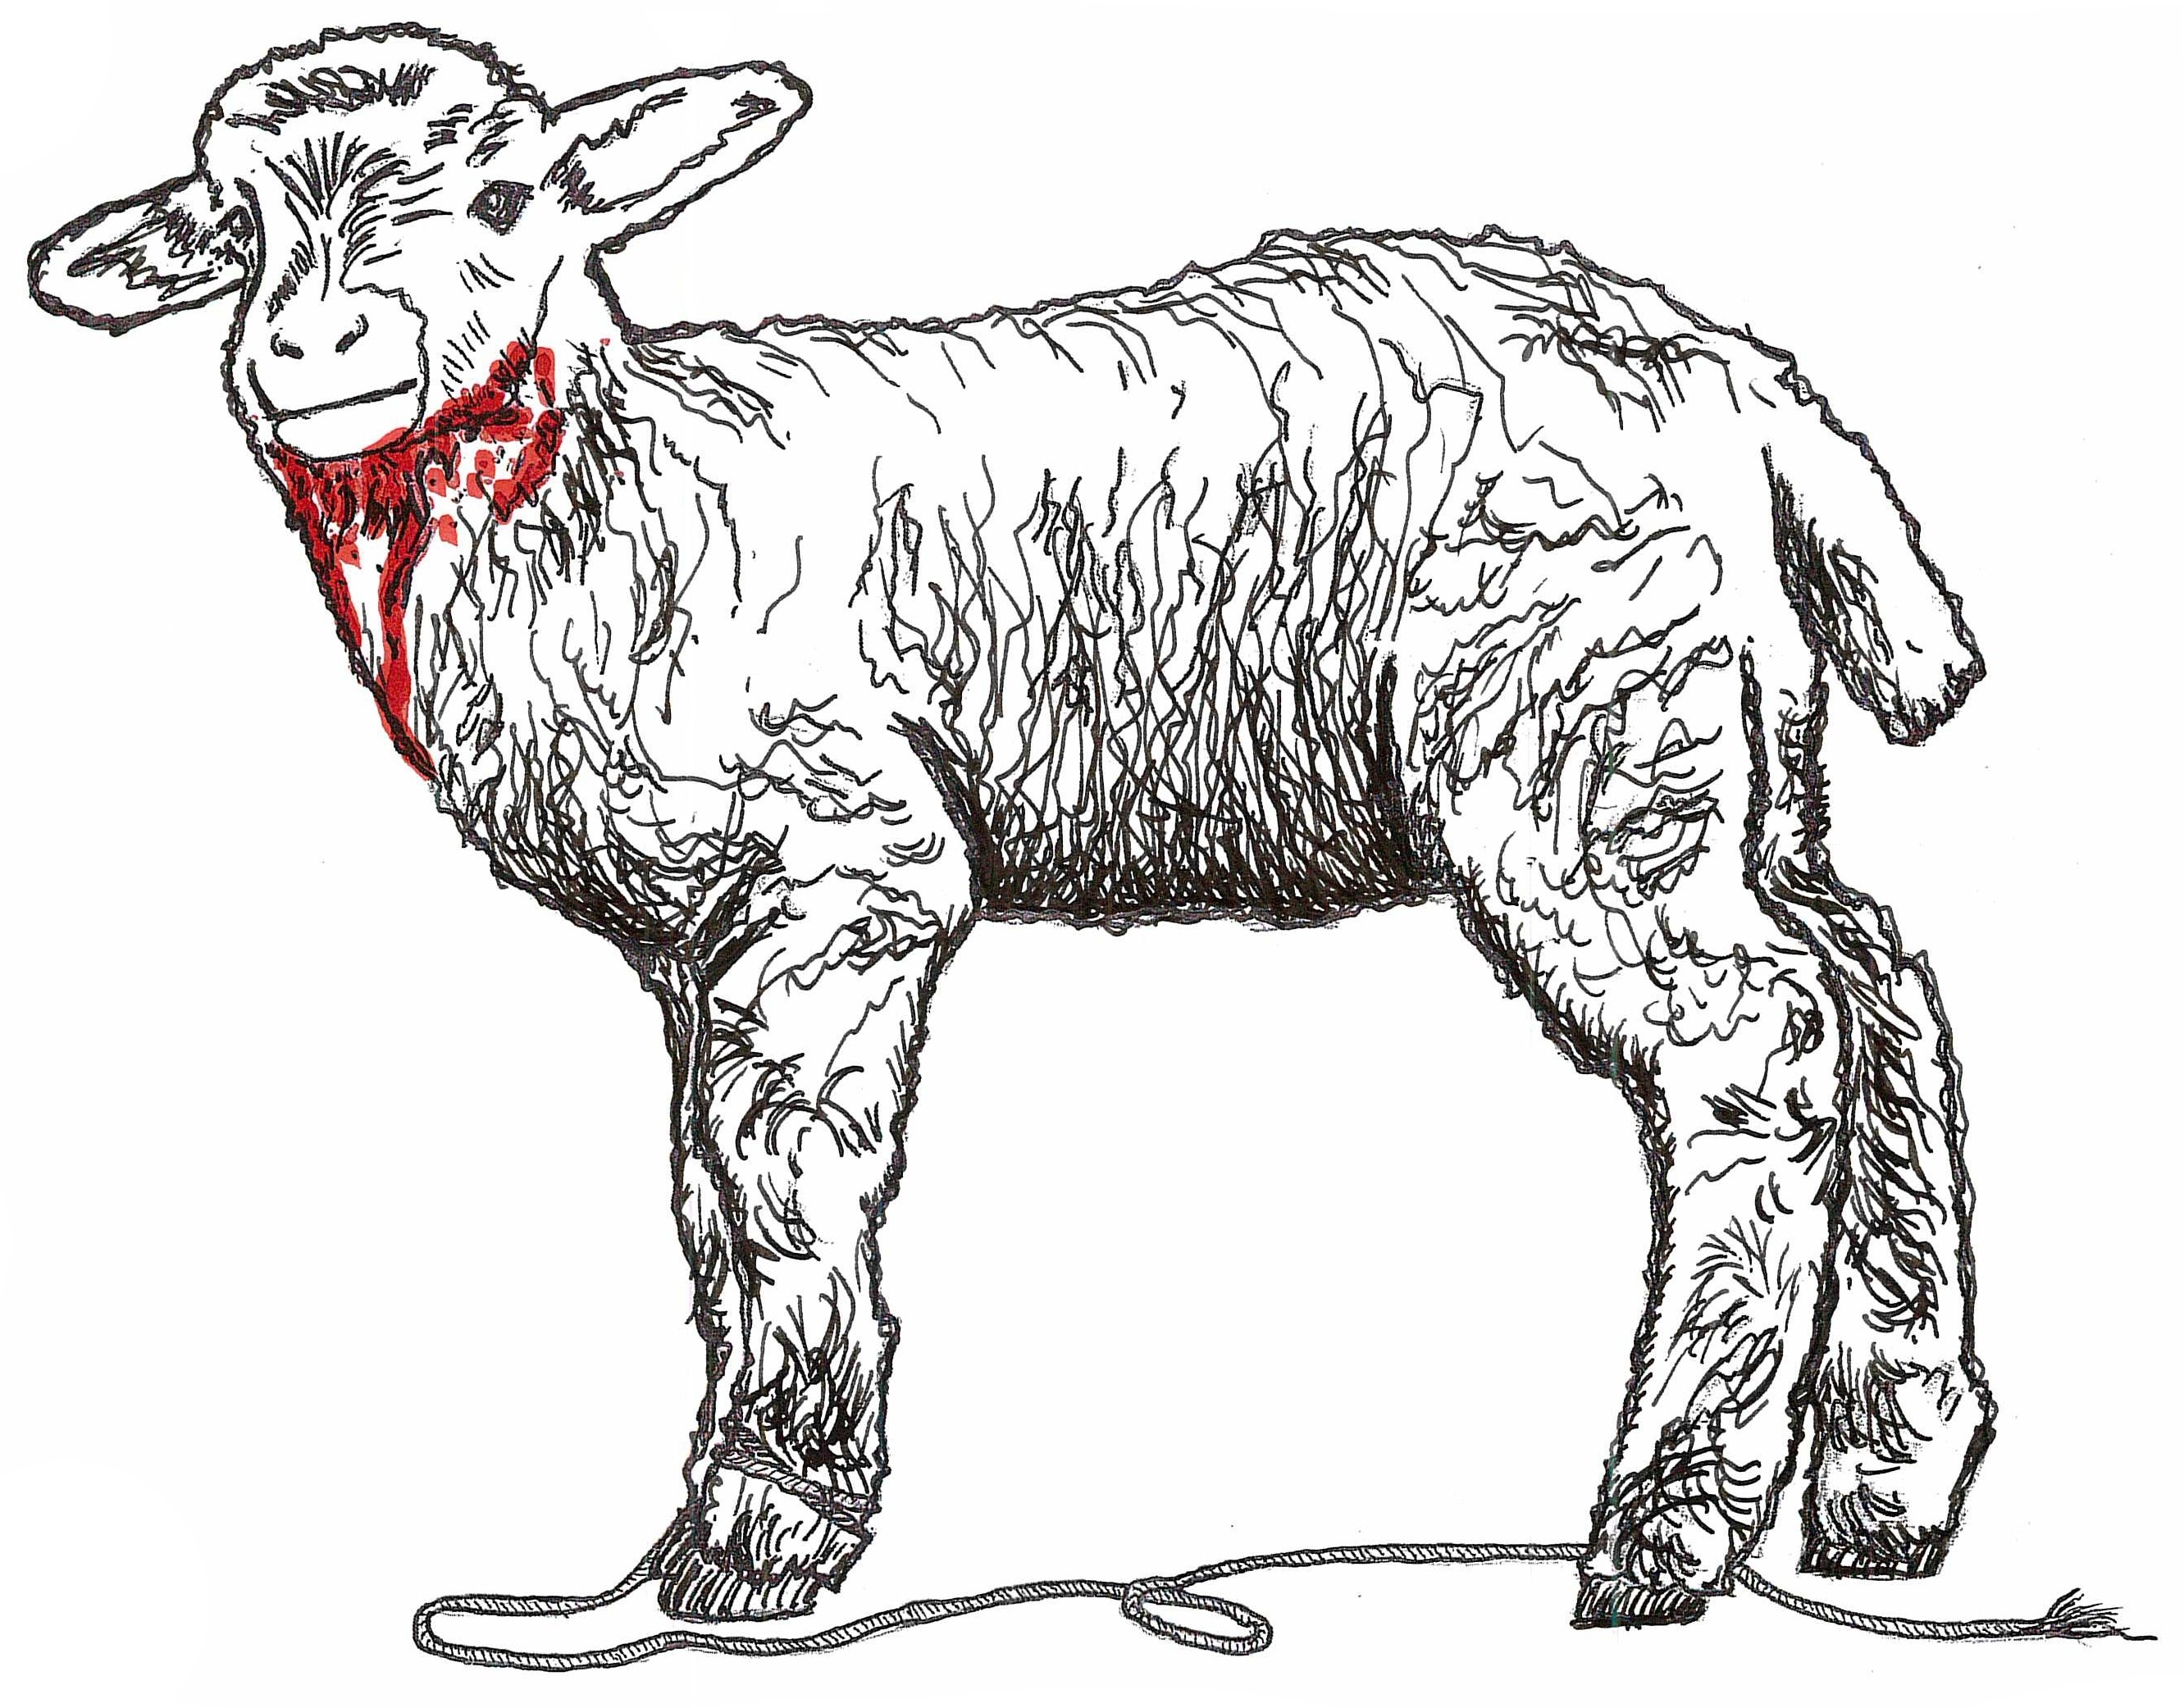
\includegraphics[width=4cm]{lamb3nooval} \\
%\vfill
\bigskip
\bigskip\bigskip

\textit{...And when I see the blood, I will pass over you...} \\ \medskip % Subtitle

March 2018\ -- version 1.4 % Time and version

\vfill
\end{center}
\end{titlepage}
    
\end{document}
